\documentclass[10pt]{beamer}
\usepackage{amsmath,amsfonts}	% use math symbols
\usepackage{graphicx} % insert images
\usepackage{url} % insert urls
\usepackage{hyperref}
\usepackage{amsthm}
\usepackage{auto-pst-pdf}
\setbeamertemplate{navigation symbols}{}
\usepackage{listings}
\usepackage{xcolor}
\usepackage{moresize}

\definecolor{cream}{rgb}{1.0, 0.99, 0.82}

\lstset{frame=single, basicstyle=\color{black}\ttfamily\ssmall, backgroundcolor=\color{cream}}



%%%%%%%%%%%%%%%%%%%%%%%%%%%%%%%%%%%%%%%%%%%%



\begin{document}

\title{A Brief Introduction to Git}
\author{Hautahi Kingi}
\date{}


\maketitle

%%%%%%%%%%%%%%%%%%%%%%%%%%%%%%%%%%%%
\begin{frame}{Introduction}


Version control is better than mailing files back and forth because:
\begin{itemize}
\item
Nothing that is committed to version control is ever lost. It's always possible to go back in time to see exactly who wrote what on a particular day, or what version of a program was used to generate a particular set of results.
\item
It keeps a record of who made what changes when, so that if people have questions later on, they know who to ask.
\item
It's hard (but not impossible) to accidentally overlook or overwrite someone's changes: the version control system automatically notifies users whenever there's a conflict between one person's work and another's.
\end{itemize}
Git is one of many version control systems. It is more complex than some alternatives, but it is widely used, both because it's easy to set up and because of a hosting site called GitHub, which we will get to later.

\end{frame}

%%%%%%%%%%%%%%%%%%%%%%%%%%%%%%%%%%%%
\begin{frame}[fragile]{Set Up}

After downloading Git, an easy way to check if it is installed and working properly is
\begin{lstlisting}
$ git help
\end{lstlisting}
On our first time with Git on a new machine, we need to do a few things.
\begin{lstlisting}
$ git config --global user.name "Hautahi Kingi"
$ git config --global user.email "hrk55@cornell.edu"
$ git config --global color.ui "auto"
$ git config --global core.editor "nano"
\end{lstlisting}
Navigate to the my\_thesis folder that we created earlier (see command line slides).
\begin{lstlisting}
$ cd my_thesis
\end{lstlisting}
and tell git to make it a \emph{repository}. A repository is a storage area where a version control system stores old revisions of files and information about who changed what, when.
\begin{lstlisting}
$ git init
Initialized empty Git repository in /Users/hautahikingi/my_thesis/.git/
\end{lstlisting}

\end{frame}

%%%%%%%%%%%%%%%%%%%%%%%%%%%%%%%%%%%%
\begin{frame}[fragile]{The .git subdirectory}

Let's take a look at our new directory
\begin{lstlisting}
$ ls
code.m	introduction.txt
\end{lstlisting}
It looks like nothing has changed. But \emph{ls} only lists files which are not hidden. The \emph{init} command created a hidden directory, which we can see by using the -a flag
\begin{lstlisting}
$ ls -a
code.m	 .git	introduction.txt
\end{lstlisting}
Git stores information about the project in this special .git sub-directory. If deleted, we lose the project's entire history.\\

\end{frame}

%%%%%%%%%%%%%%%%%%%%%%%%%%%%%%%%%%%%
\begin{frame}[fragile]{Git Status}

\begin{lstlisting}
$ git status
On branch master

Initial commit

Untracked files:
  (use "git add <file>..." to include in what will be committed)

	code.m
	introduction.txt

nothing added to commit but untracked files present (use "git add" to track)
\end{lstlisting}
The output states that we are located on the master branch (more on this later). The \emph{Initial commit} message states that we are yet to make a commit. The \emph{Untracked files} message means that there are files in the directory that Git is not keeping track of.
\end{frame}

%%%%%%%%%%%%%%%%%%%%%%%%%%%%%%%%%%%%
\begin{frame}[fragile]{Git Add}
We tell Git to stage untracked/modified files using \emph{git add}:

\begin{lstlisting}
$ git add code.m introduction.txt
\end{lstlisting}
and checking the status again...
\begin{lstlisting}
$ git status
On branch master

Initial commit

Changes to be committed:
  (use "git rm --cached <file>..." to unstage)

	new file:   code.m
	new file:   introduction.txt
\end{lstlisting}
... tells us that Git knows that it needs to keep track of the files \emph{code.m} and \emph{introduction.txt}. But it has not yet recorded the changes. 

\end{frame}

%%%%%%%%%%%%%%%%%%%%%%%%%%%%%%%%%%%%
\begin{frame}[fragile]{Git Commit}
Let's \emph{commit} the added changes.
\begin{lstlisting}
$ git commit -m "First draft introduction and code"
[master (root-commit) 1ec0eef] First draft introduction and code
 2 files changed, 8 insertions(+)
 create mode 100755 code.m
 create mode 100644 introduction.txt
\end{lstlisting}
\begin{itemize}
\item
Git takes everything we have told it to save by using \emph{git add} and stores a copy permanently inside the special .git directory.
\item
Version has a short identifier 1ec0eef.
\item
 -m flag to record a comment that will help us remember later on what we did and why.
\end{itemize}
Now let's check the status again
\begin{lstlisting}
$ git status
On branch master
nothing to commit, working directory clean
\end{lstlisting}
This is the nice clean message that tells us everything is up to date and committed.

\end{frame}

%%%%%%%%%%%%%%%%%%%%%%%%%%%%%%%%%%%%
\begin{frame}[fragile]{Adding new Files}

Let's create a latex file called template.tex.
\begin{lstlisting}
$ ls
code.m              template.aux        template.pdf        template.tex
draft.txt           template.log        template.synctex.gz
\end{lstlisting}
My particular latex compiler created a number of auxiliary files. Checking the status of the repository gives
\begin{lstlisting}
$ git status
On branch master
Untracked files:
  (use "git add <file>..." to include in what will be committed)

	template.aux
	template.log
	template.pdf
	template.synctex.gz
	template.tex

nothing added to commit but untracked files present (use "git add" to track)
\end{lstlisting}
The \emph{template} files are untracked because I have not added them.

\end{frame}

%%%%%%%%%%%%%%%%%%%%%%%%%%%%%%%%%%%%
\begin{frame}[fragile]{Git ignore}

I don't particularly care about the auxiliary latex files. They are a waste of disk space and distract us from changes that actually matter. We can tell Git to ignore them by creating a file in the root directory of our project called .gitignore.
\begin{lstlisting}
$ nano .gitignore
\end{lstlisting}
\begin{center}
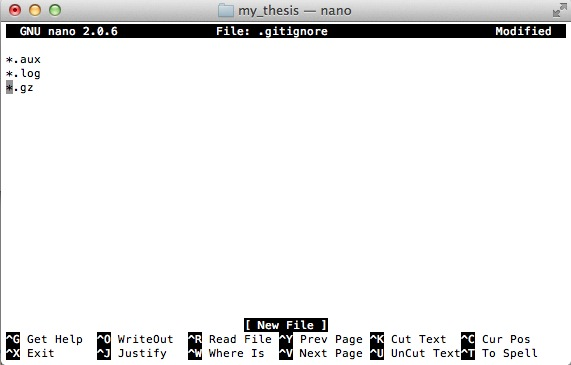
\includegraphics[width=5cm]{./auxfiles/gitignore.jpg}
\end{center}
We've told Git to ignore any file whose name ends in .aux, .log and .gz. 
\end{frame}

%%%%%%%%%%%%%%%%%%%%%%%%%%%%%%%%%%%%
\begin{frame}[fragile]{Git ignore}
Once we have created the .gitignore file, the output of git status is much cleaner:
\begin{lstlisting}
$ git status
On branch master
Untracked files:
  (use "git add <file>..." to include in what will be committed)

	.gitignore
	template.pdf
	template.tex

nothing added to commit but untracked files present (use "git add" to track)
\end{lstlisting}
Git no longer notices those pesky auxiliary latex files and we can focus on the changes that matter.

\end{frame}

%%%%%%%%%%%%%%%%%%%%%%%%%%%%%%%%%%%%
\begin{frame}[fragile]{Modifying files}

Now let's edit our introduction.txt file and check the status again.
\begin{lstlisting}
$ nano introduction.txt
$ cat intoduction.txt
We were wanderers from the beginning.
We knew every stand of tree for a hundred miles.
$ git status
On branch master
Changes not staged for commit:
  (use "git add <file>..." to update what will be committed)
  (use "git checkout -- <file>..." to discard changes in working directory)

	modified:   introduction.txt

Untracked files:
  (use "git add <file>..." to include in what will be committed)

	.gitignore
	template.pdf
	template.tex

no changes added to commit (use "git add" and/or "git commit -a")
\end{lstlisting}

As well as the untracked files in the previous status check, Git also tells us that the introduction.txt file has been modified.

\end{frame}

%%%%%%%%%%%%%%%%%%%%%%%%%%%%%%%%%%%%
\begin{frame}[fragile]{Completing the Git Cycle}
 Let's now add and commit these changes.
\begin{lstlisting}
$ git add introduction.txt template.tex template.pdf .gitignore
$ git status
On branch master
Changes to be committed:
  (use "git reset HEAD <file>..." to unstage)

	new file:   .gitignore
	modified:   introduction.txt
	new file:   template.pdf
	new file:   template.tex
$ git commit -m "New latex file and added line to introduction.txt"
[master d796846] New latex file and added line to introduction.txt
 4 files changed, 49 insertions(+)
 create mode 100644 .gitignore
 create mode 100644 template.pdf
 create mode 100644 template.tex
\end{lstlisting}
and checking the status....
\begin{lstlisting}
$ git status
On branch master
nothing to commit, working directory clean
\end{lstlisting}
... we're back to a clean sheet.


\end{frame}

%%%%%%%%%%%%%%%%%%%%%%%%%%%%%%%%%%%%
\begin{frame}[fragile]{An overview of the Git Cycle}


We should now be able to see the basic structure of how Git works. Once a directory is set up as a Git repository using \emph{git init}, any change that we make to that directory is noted by Git. The workflow is then as follows:
\begin{enumerate}
\item
Modify/create new folders and files.
\item
Stage these changes ready to commit by using \emph{git add}.
\item
Commit the changes using \emph{git commit} which permanently saves the current version of that repository.
\end{enumerate}

\end{frame}

%%%%%%%%%%%%%%%%%%%%%%%%%%%%%%%%%%%%
\begin{frame}[fragile]{GitHub: Taking Version Control Online}


Version control really comes into its own when we begin to collaborate with other people. In practice, a remote repository stored on a central hub is preferable to one stored on someone's laptop. For this reason, websites like Github and BitBucket are becoming increasingly popular.\\~\\

Login to your profile page on GitHub. Click on the icon in the top right corner to create a new repository called my\_thesis.
\begin{center}
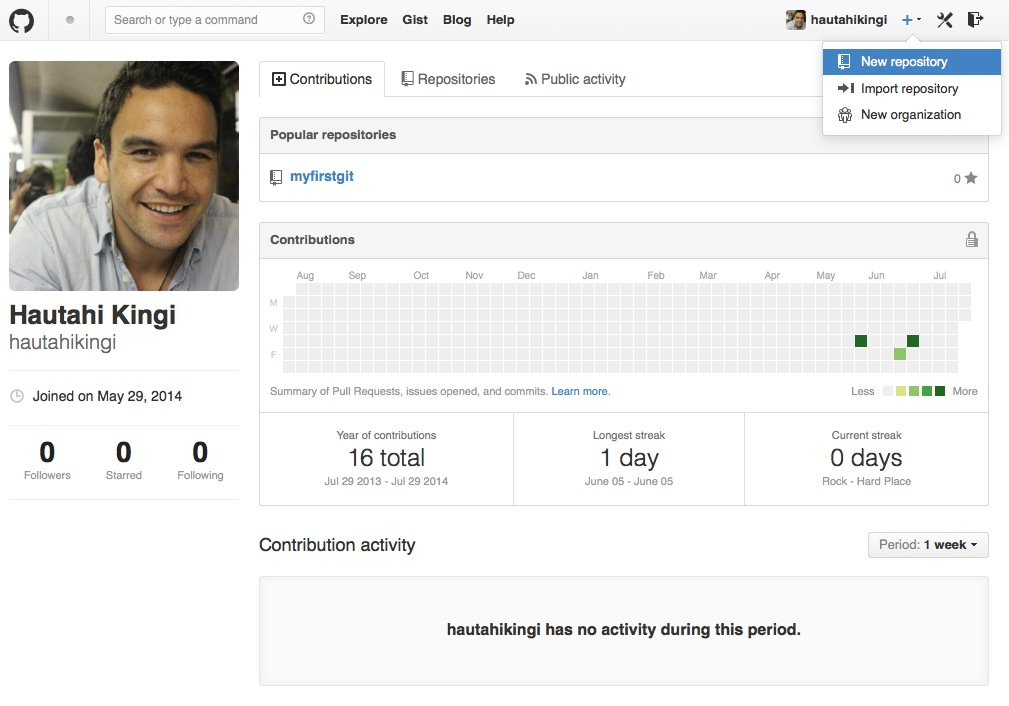
\includegraphics[width=5cm]{./auxfiles/Ghub.jpg}
\end{center}
Public repositories allow any Github user to access your files. A student account receives 5 free private repositories.

\end{frame}

%%%%%%%%%%%%%%%%%%%%%%%%%%%%%%%%%%%%
\begin{frame}[fragile]{Creating an Online Repository}

\begin{center}
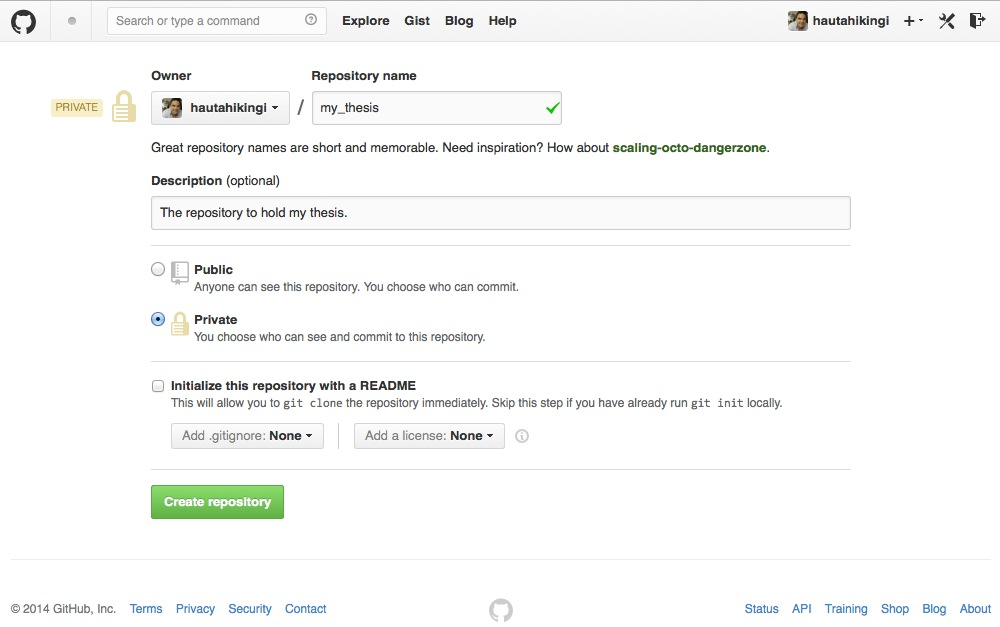
\includegraphics[width=5cm]{./auxfiles/Ghub1.jpg}
\end{center}
Clicking the green button creates a repository on the Github website. Once created, GitHub displays a page with a URL and some information on how to configure your local repository. 
\begin{center}
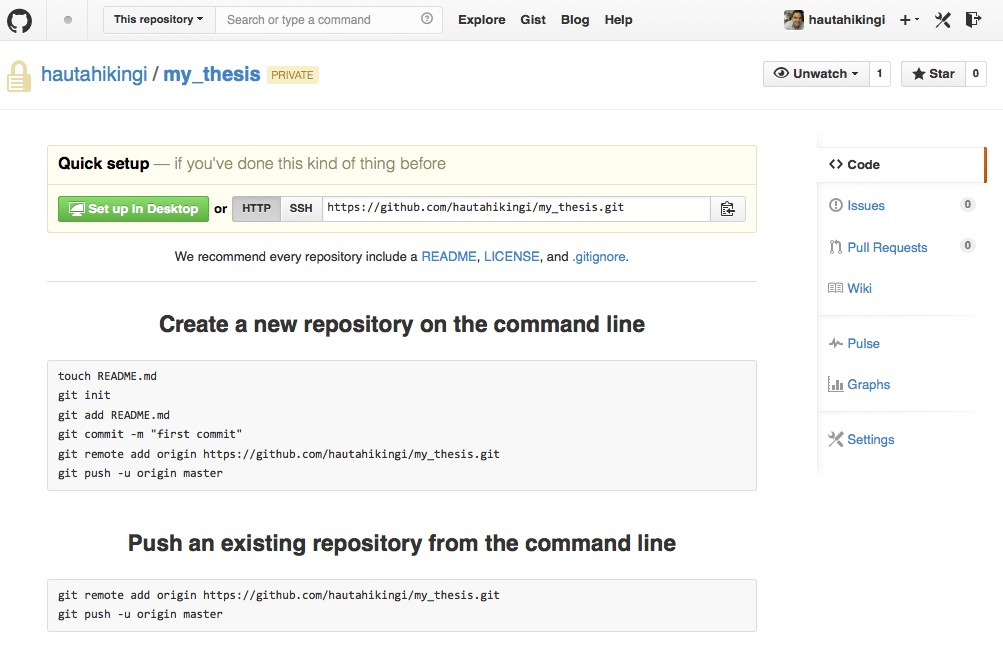
\includegraphics[width=5cm]{./auxfiles/Ghub2.jpg}
\end{center}
\end{frame}

%%%%%%%%%%%%%%%%%%%%%%%%%%%%%%%%%%%%
\begin{frame}[fragile]{Connecting Local and Online Repositories}

The home page of the GitHub repository includes instructions on how to link our newly created repository with our local repository.  We are interested in the instructions in the second box.\\~\\

Making sure we are in the my\_thesis directory locally...
\begin{lstlisting}
$ git remote add origin https://github.com/hautahikingi/my_thesis.git
\end{lstlisting}
This command tells git to add a remote named \emph{origin} at the url \emph{https://github.com/hautahikingi/my\_thesis.git}.\\~\\

We can check that the command worked by typing
\begin{lstlisting}[frame=single]
$ git remote -v
origin	https://github.com/hautahikingi/my_thesis.git (fetch)
origin	https://github.com/hautahikingi/my_thesis.git (push)
\end{lstlisting}
which lists all remote repositories. The -v flag is short for verbose which tells git to show the remote url as well as the nickname.\\

\end{frame}

%%%%%%%%%%%%%%%%%%%%%%%%%%%%%%%%%%%%
\begin{frame}[fragile]{Pushing}

So far all we have done is set up a remote repository and linked it to our local repository. But if we take a look at our remote repository, it is still empty. We fix this by pushing the changes from our local repository to the GitHub repository
\begin{lstlisting}
$ git push origin master
\end{lstlisting}
It will sometimes ask for your username and password
\begin{lstlisting}[frame=single]
Username for 'https://github.com': hautahikingi
Password for 'https://hautahikingi@github.com':
\end{lstlisting}
When you are typing in your password the cursor won't move. Don't panic just type it out and press enter.
\begin{lstlisting}[frame=single]
Counting objects: 10, done.
Delta compression using up to 4 threads.
Compressing objects: 100\% (8/8), done.
Writing objects: 100\% (10/10), 42.65 KiB | 0 bytes/s, done.
Total 10 (delta 1), reused 0 (delta 0)
To https://github.com/hautahikingi/my_thesis.git
 * [new branch]      master -> master
Branch master set up to track remote branch master from origin.
\end{lstlisting}

\end{frame}


%%%%%%%%%%%%%%%%%%%%%%%%%%%%%%%%%%%%
\begin{frame}[fragile]{GitHub - a visual repository}
The homepage for our remote repository confirms that it is now linked to our local repository.
\begin{center}
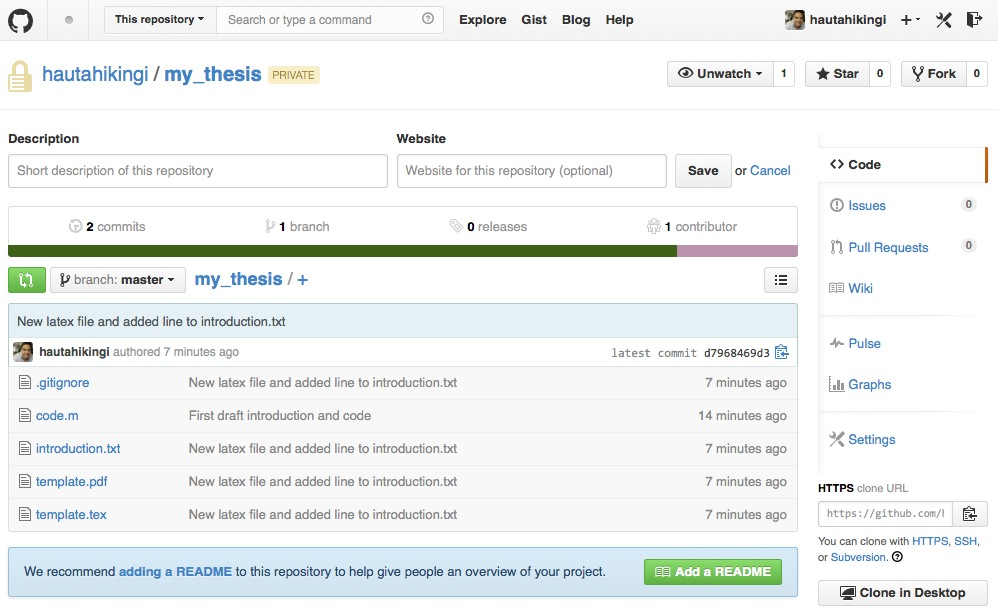
\includegraphics[width=5cm]{./auxfiles/Ghub3.jpg}
\end{center}
Selecting \emph{Networks} from the \emph{Graphs} tab on the right...

\begin{center}
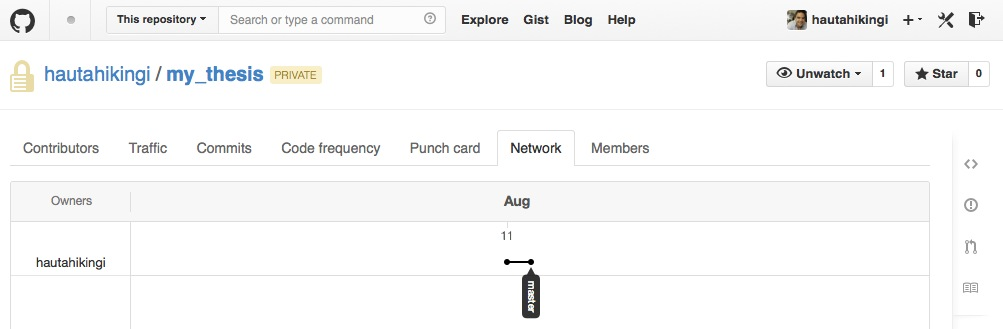
\includegraphics[width=5cm]{./auxfiles/Network.jpg}
\end{center}
... gives a visual representation of the evolution of the repository. Each commit is represented by a node in the graph. There are two nodes because we have performed two commits.




\end{frame}

%%%%%%%%%%%%%%%%%%%%%%%%%%%%%%%%%%%%
\begin{frame}[fragile]{Centralized vs Distributed Version Control Systems}

Version control systems are often divided into two groups: �centralized� and �distributed�.\\~\\

Centralized version control systems, such as subversion, are based on the idea that there is a single �central� copy of your project on a server, and programmers \emph{commit} their changes to this central copy.\\~\\

The basic workflow is to pull down any changes other people have made from the central server. Then make your changes and commit these to the central server.\\~\\

Git is a Distributed VCS. These do not necessarily rely on a central server to store all versions of a project�s files. Instead, every developer \textbf{clones} a copy of a repository and has the full history of the project on their own hard drive. This copy has all of the metadata of the original.\\~\\

So instead of a central repository being required, it is now optional and purely a matter of preference.\\~\\





\end{frame}
%%%%%%%%%%%%%%%%%%%%%%%%%%%%%%%%%%%%
\begin{frame}[fragile]{Centralized vs Distributed Version Control Systems}

We have already made use of some of the features of a DVCS.\\~\\

We were able to commit changes locally even before we created the central remote repository.\\~\\

Once we pushed our local copy to the remote repository, GitHub still registered each separate commit (two in our case). This is one of the main advantages of distributed systems. Centralized systems only record commits that are made directly to the remote repository. For example, in subversion, there would only be one node in our network tree.\\~\\

Being able to commit locally is advantageous for a number of reasons. First, performing actions is extremely fast because Git only needs to access the hard drive, not a remote server (except for pushing and pulling of course).\\~\\

Everything but pushing and pulling can be done without an internet connection. So you can work on a plane, and you won�t be forced to commit several bugfixes as one big changeset.\\~\\


\end{frame}

%%%%%%%%%%%%%%%%%%%%%%%%%%%%%%%%%%%%
\begin{frame}[fragile]{Pulling}


We can pull changes from the remote repository to the local one as well:

\begin{lstlisting}
$ git pull origin master
From https://github.com/hautahikingi/my_thesis
 * branch            master     -> FETCH_HEAD
Already up-to-date.
\end{lstlisting}
Pulling has no effect in this case because the two repositories are already synchronized. If someone else had pushed some changes to the repository on GitHub, though, this command would download them to our local repository.\\

\end{frame}

%%%%%%%%%%%%%%%%%%%%%%%%%%%%%%%%%%%%
\begin{frame}[fragile]{Cloning}
We can simulate working with a collaborator using another copy of the repository on our local machine. To do this, \emph{cd} to another directory on your computer. Instead of creating a new repository here with \emph{git init}, we will \textbf{clone} the existing repository from GitHub.
\begin{lstlisting}
$ cd /Users/hautahikingi/Dropbox/temporary
$ git clone https://github.com/hautahikingi/my_thesis.git
Cloning into 'my_thesis'...
remote: Counting objects: 10, done.
remote: Compressing objects: 100\% (7/7), done.
remote: Total 10 (delta 1), reused 10 (delta 1)
Unpacking objects: 100\% (10/10), done.
Checking connectivity... done.
\end{lstlisting}
I navigated to a new folder called \emph{temporary} and then created a fresh local copy of a remote repository. Our computer now has two copies of the repository.

\end{frame}

%%%%%%%%%%%%%%%%%%%%%%%%%%%%%%%%%%%%
\begin{frame}[fragile]{Working with a collaborator}
Let's make a change to the copy in \emph{/temporary/my\_thesis}:
\begin{lstlisting}
$ cd my_thesis
$ nano introduction.txt
$ cat introduction.txt
We were wanderers from the beginning.
We knew every stand of tree for a hundred miles.
The frontier was everywhere.
\end{lstlisting}
and now let's add and commit
\begin{lstlisting}
$ git add introduction.txt
$ git commit -m "Added a third line to introduction.txt"
[master 2b1b130] Added a third line to introduction.txt
 1 file changed, 1 insertion(+)
\end{lstlisting}
and checking the status...
\begin{lstlisting}
$ git status
On branch master
Your branch is ahead of 'origin/master' by 1 commit.
  (use "git push" to publish your local commits)

nothing to commit, working directory clean
\end{lstlisting}
This message tells us that we have committed all changes, but that we have not yet pushed these changes to the remote repository on Github. Again, this is a feature of \textbf{distributed} version control systems.\\


\end{frame}

%%%%%%%%%%%%%%%%%%%%%%%%%%%%%%%%%%%%
\begin{frame}[fragile]{Working with a collaborator}

Let's now push the change to Github
\begin{lstlisting}
$ git push origin master
Counting objects: 5, done.
Delta compression using up to 4 threads.
Compressing objects: 100\% (3/3), done.
Writing objects: 100\% (3/3), 345 bytes | 0 bytes/s, done.
Total 3 (delta 1), reused 0 (delta 0)
To https://github.com/hautahikingi/my_thesis.git
   170ae6f..3cafe3a  master -> master
\end{lstlisting}
Checking the status...
\begin{lstlisting}
$ git status
On branch master
Your branch is up-to-date with 'origin/master'.

nothing to commit, working directory clean
\end{lstlisting}
This tells us that we have committed all changes, and that this is also reflected in the remote repository.


\end{frame}

%%%%%%%%%%%%%%%%%%%%%%%%%%%%%%%%%%%%
\begin{frame}[fragile]{Working with a collaborator}
The network map also confirms this...
\begin{center}
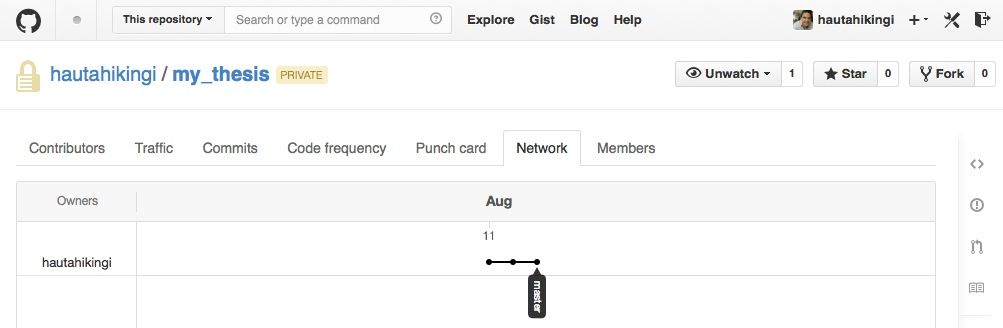
\includegraphics[width=5cm]{./auxfiles/Network_update.jpg}
\end{center}
We can now download changes into the original repository on our machine:
\begin{lstlisting}
$ cd /Users/hautahikingi/Dropbox/my_thesis
$ git pull origin master
remote: Counting objects: 3, done.
remote: Compressing objects: 100\% (1/1), done.
remote: Total 3 (delta 2), reused 3 (delta 2)
Unpacking objects: 100\% (3/3), done.
From https://github.com/hautahikingi/my_thesis
 * branch            master     -> FETCH_HEAD
   d796846..2b1b130  master     -> origin/master
Updating d796846..2b1b130
Fast-forward
 introduction.txt | 1 +
 1 file changed, 1 insertion(+)
\end{lstlisting}
Both our local repositories are now in sync with the remote repository. In practice, we would never have two copies of the same remote repository on our laptop at once.
\end{frame}

%%%%%%%%%%%%%%%%%%%%%%%%%%%%%%%%%%%%
\begin{frame}[fragile]{An ECCO Example}
Pushing and pulling changes gives us a reliable way to share work between different people and machines.\\~\\

Login to ECCO and clone the remote repository from the terminal.

\begin{center}
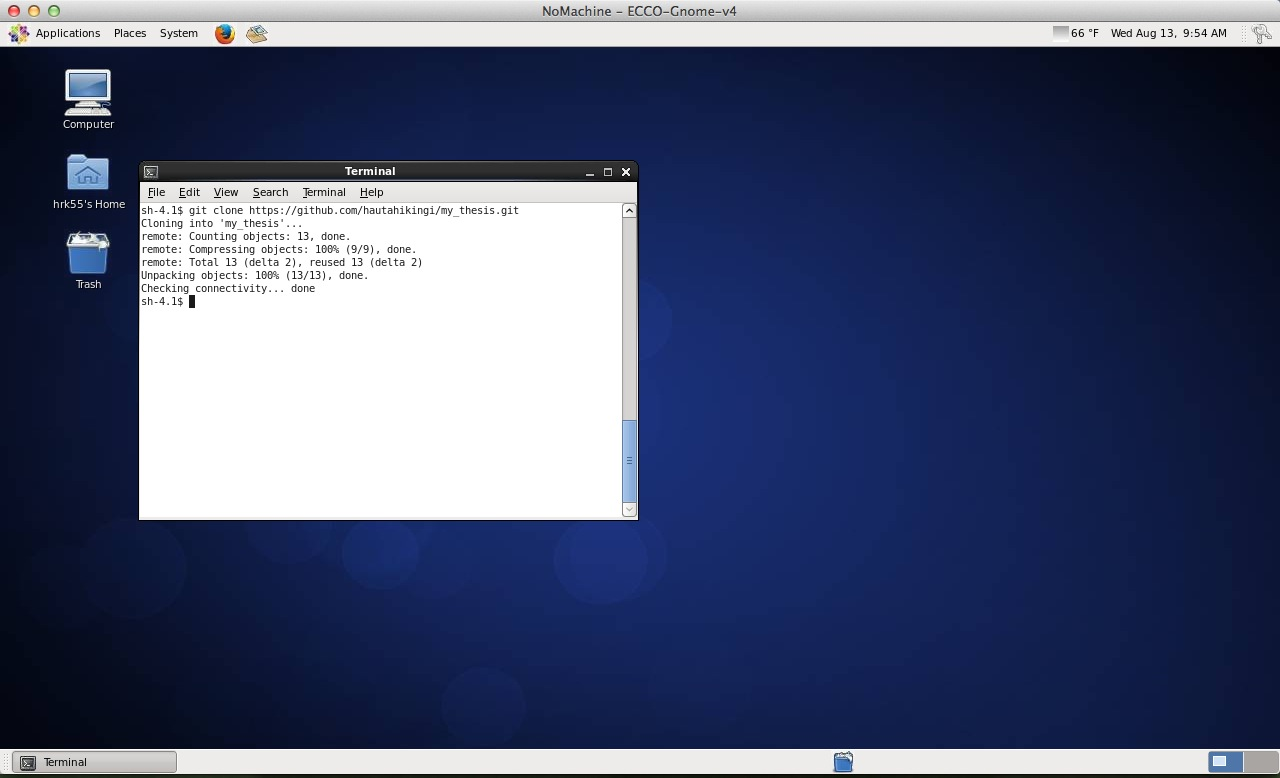
\includegraphics[width=10cm]{./auxfiles/ECCO.jpg}
\end{center}



\end{frame}

%%%%%%%%%%%%%%%%%%%%%%%%%%%%%%%%%%%%
\begin{frame}[fragile]{An ECCO Example}

Now create some changes, add and commit.
\begin{lstlisting}
$ cd my_thesis
$ nano conclusion.txt
$ cat conclusion.txt
Herman Melville, in Moby Dick, spoke for wanderers in all epochs and meridians:
"I am tormented with an everlasting itch for things remote. I love to sail
forbidden seas..." 
$ git add conclusion.txt
$ git commit -m "Began conclusion.txt"
[master ac717a9] Began conclusion.txt
 Committer: hrk55 <hrk55@ecco.vrdc.cornell.edu>
Your name and email address were configured automatically based
on your username and hostname. Please check that they are accurate.
You can suppress this message by setting them explicitly:

    git config --global user.name "Your Name"
    git config --global user.email you@example.com

After doing this, you may fix the identity used for this commit with:

    git commit --amend --reset-author

 1 file changed, 3 insertions(+)
 create mode 100644 conclusion.txt
\end{lstlisting}
Because I have not configured my Git settings on the ECCO server, Git has assigned me a different username.





\end{frame}

%%%%%%%%%%%%%%%%%%%%%%%%%%%%%%%%%%%%
\begin{frame}[fragile]{An ECCO Example}
Let's now push the changes to our remote repository.

\begin{center}
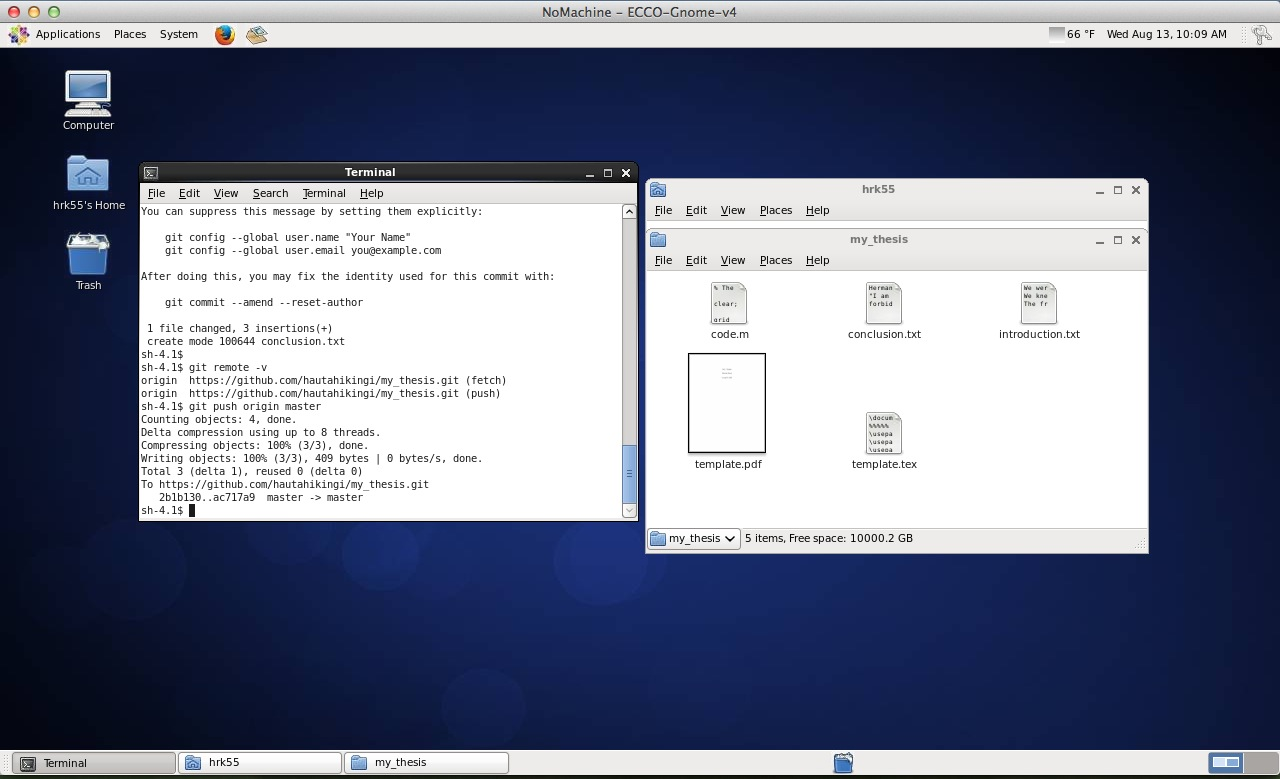
\includegraphics[width=5cm]{./auxfiles/ECCO2.jpg}
\end{center}

Switching back to your local copy we can then pull these changes.
\begin{lstlisting}
$ git pull origin master
remote: Counting objects: 3, done.
remote: Compressing objects: 100\% (2/2), done.
remote: Total 3 (delta 1), reused 3 (delta 1)
Unpacking objects: 100\% (3/3), done.
From https://github.com/hautahikingi/my_thesis
 * branch            master     -> FETCH_HEAD
   2b1b130..ac717a9  master     -> origin/master
Updating 2b1b130..ac717a9
Fast-forward
 conclusion.txt | 3 +++
 1 file changed, 3 insertions(+)
 create mode 100644 conclusion.txt
\end{lstlisting}


Used in this way, Git acts like a more robust Dropbox.

\end{frame}

%%%%%%%%%%%%%%%%%%%%%%%%%%%%%%%%%%%%
\begin{frame}[fragile]{The GitHub GUI}
There are now a number of fantastic GitHub GUIs. Let's take a quick look at the GUI created by Github itself.


\begin{center}
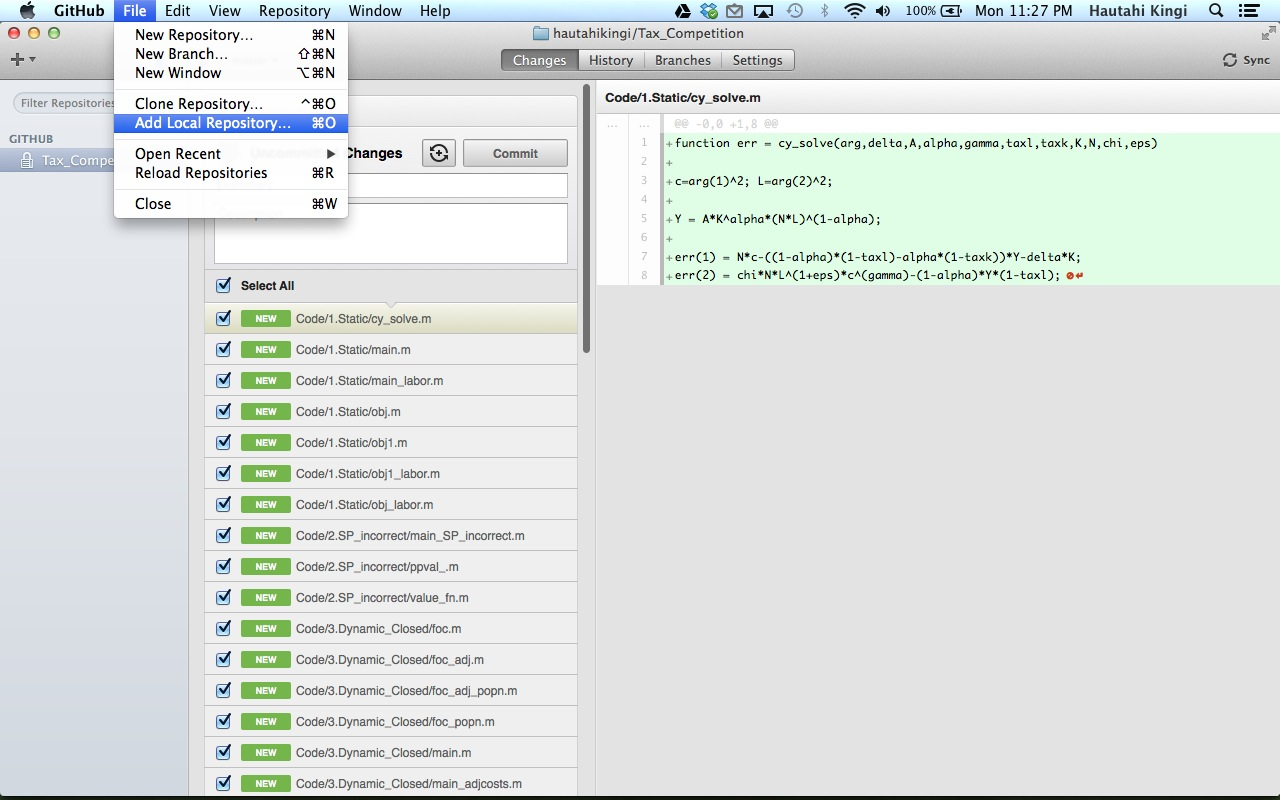
\includegraphics[width=10cm]{./auxfiles/GUI_add.jpg}
\end{center}

When we first launch the GUI we want to tell it to add our local repository from the menu.


\end{frame}
%%%%%%%%%%%%%%%%%%%%%%%%%%%%%%%%%%%%
\begin{frame}[fragile]{The GitHub GUI}
Select the repository in the left-hand menu. 
\begin{center}
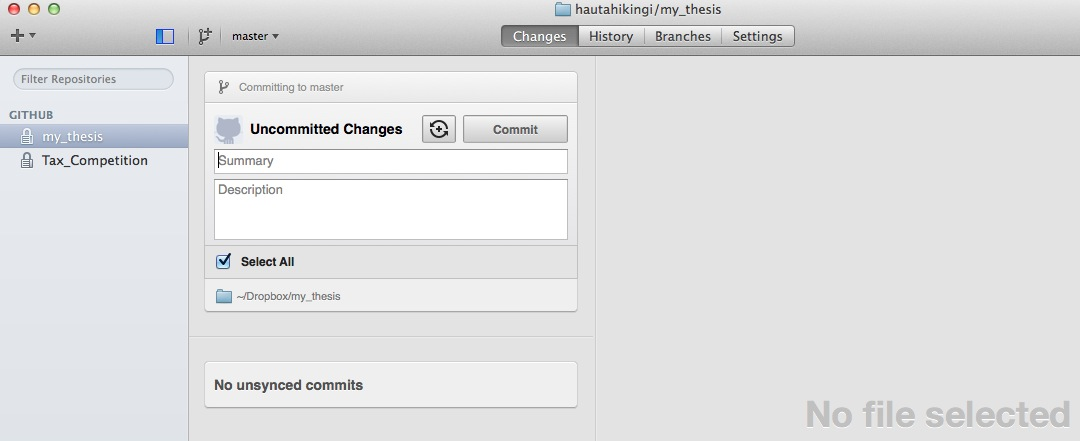
\includegraphics[width=10cm]{./auxfiles/GUI_changes.jpg}
\end{center}
The right hand pane shows a range of information about that repository contained in four separate panels. The \emph{changes} panel shows the changes made within the repository which are yet to be committed. It effectively shows the same information as typing \emph{git status} in the command line. As you can see, we have nothing untracked or changed since the last commit.

\end{frame}
%%%%%%%%%%%%%%%%%%%%%%%%%%%%%%%%%%%%
\begin{frame}[fragile]{The GitHub GUI}

The history panel allows us to select each commit, and investigate what changes were made since the last commit.
\begin{center}
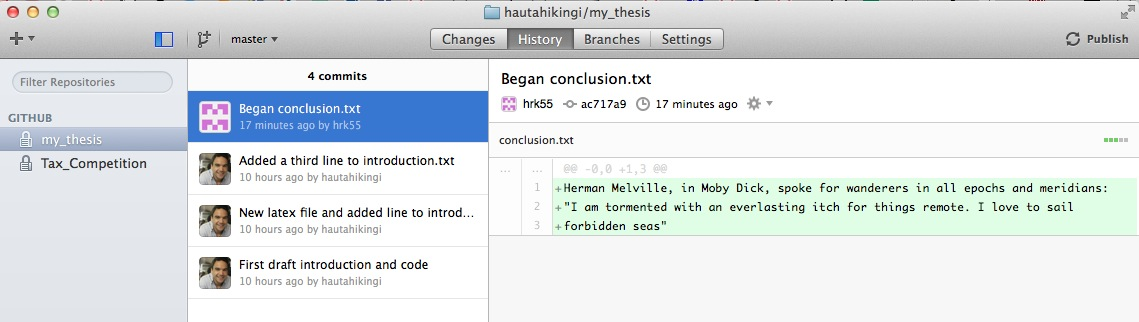
\includegraphics[width=10cm]{./auxfiles/GUI_history.jpg}
\end{center}
It provides the same information as the \emph{git log} and \emph{git diff} commands which we have not covered.


\end{frame}
%%%%%%%%%%%%%%%%%%%%%%%%%%%%%%%%%%%%
\begin{frame}[fragile]{}

Most of this material was taken from the Software Carpentry website and their excellent bootcamp. More detailed explanations of what I discuss in these notes can be found at: http://software-carpentry.org/lessons.html
\end{frame}

%%%%%%%%%%%%%%%%%%%%%%%%%%%%%%%%%%%%
\setbeamercolor{background canvas}{bg=black}
\begin{frame}[plain]{}



\end{frame}
\setbeamercolor{background canvas}{bg=white}

%%%%%%%%%%%%%%%%%%

\end{document}
